\chapter{Experiments}
\label{chapter:experiments}

This chapter presents experiments we have conducted to evaluate the viability of Bayesian optimization. All of the cases are examples of optimizing neural networks, because that is the area of interest of this work.

We present one example from reinforcement learning, specifically the REINFORCE algorithm \citep{suttonbarto2018reinforcement}, as an example of a smaller and simpler network. In this settings, we also compare Bayesian optimization with a random search. Next we show a larger experiment where we train a recurrent neural network \citep{dlbook}, specifically a tagger, on a SIGMORPHON 2019 shared task \citep{sigmorphon2019task2}, where the network is trained on a significantly larger dataset in multiple languages. Lastly, we show two smaller examples, one of a tokenizer written in C++, and second a network for speech recognition.

\section{REINFORCE}
\label{section:experiments-empirical-bayes}

\begin{figure}[t]
	\begin{center}
		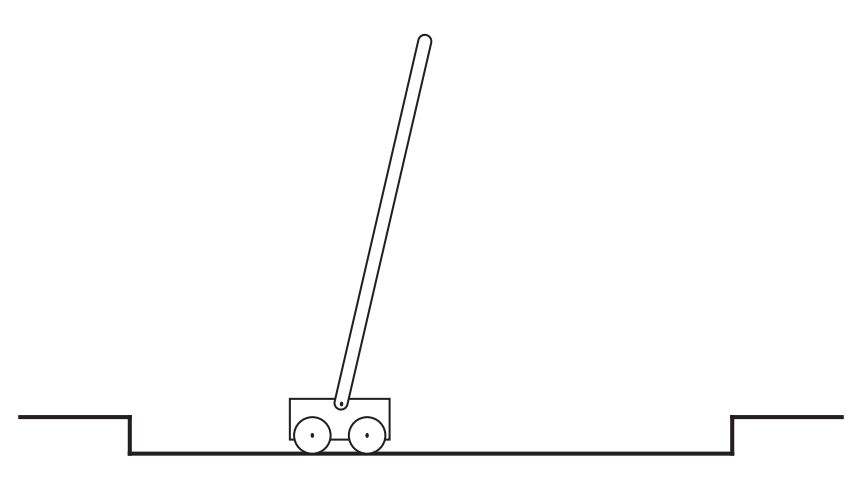
\includegraphics[width=1.0\textwidth]{images/cartpole.png}
		\caption{The objective of the task is to balance the pole on top of a cart moving along
			a track. A failure occurs if the pole falls beyond a certain angle, and the agent
			is rewarded $+1$ for every time step when the pole has not fallen over.}
		\label{figure:cartpole}
	\end{center}
\end{figure}

In order to evaluate the effectiveness of Bayesian optimization and compare it to random search, we chose the REINFORCE algorithm on a simple task in reinforcement learning, because the network is small and fast to train, but at the same time sensitive to hyperparameters. The goal of the agent is to balance a pole on top of a cart by moving either left or right, as shown in \autoref{figure:cartpole}. For each time step when the pole has not fallen over the agent receives $+1$ reward, up to a maximum of $500$. Because an episode can end rather quickly when the agent performs a few bad actions, some combinations of hyperparameters results in very low values of the objective function (e.g., $< 50$). On the other hand, reaching the perfect $500$ reward is not very difficult after some exploration of the search space. Out of our $60$ different runs of the experiment, only one was not able to find the perfect score in the allotted $50$ evaluations of the objective function.

Overall, we repeated the experiment three times. Once purely with a random search, once with a non-informative prior, and once with an informative prior, where the mean was set to the mean of the hyperparameter range (per hyperparameter) and standard deviation to a quarter of the range. Each of these setups was then executed $20$ times, each with $50$ evaluations of the objective function. Because of the noisy aspect of reinforcement learning, we modified the objective function so that instead of training and evaluating the network once, we trained it yet another $20$ times from scratch, evaluated each separately, and reported the average objective achieved. Therefore, if the optimizer receives an objective value of $500$, then all $20$ of the sub-evaluations managed to reach that score.

We show the numeric results in \autoref{table:reinforce-results}. The \emph{AUC} column measures the area under the convergence plot (see \autoref{figure:convergence-plot}), specifically the area under the cumulative maximum. The value was then normalized so that it would be $1$ exactly when a score of $500$ was achieved on the first sample. We also report the mean $\mu_{\text{time to max}}$ and standard deviation $\sigma_{\text{time to max}}$ of the time (number of evaluations) it take the optimizer to achieve the score of $500$.

\begin{table}[t]
	\begin{center}
		\begin{tabular}{||c c c c||} 
			\hline
			Optimizer & AUC & $\mu_{\text{time to max}}$ & $\sigma_{\text{time to max}}$ \\ [0.5ex] 
			\hline\hline
			Random Search & $0.89$ & $19.35$ & $15.73$ \\ 
			\hline
			Non-informative Prior & $0.91$ & $12.75$ & $10.73$ \\
			\hline
			Informative Prior & $0.90$ & $12.25$ & $9.74$  \\
			\hline
		\end{tabular}
		\caption{Results of a random search and Bayesian optimization with a non-informative and informative priors on the cart-pole balancing task.}
		\label{table:reinforce-results}
	\end{center}
\end{table}

Intuitively, the $\mu_{\text{time to max}}$ shows how fast the optimizer is able to find the maximum of the objective function, and $\sigma_{\text{time to max}}$ measures its consistency. The results clearly show that Bayesian optimization as compared to a random search is almost twice as fast at finding the maximum, and also achieves lower variance.

\begin{figure}
	\begin{center}
		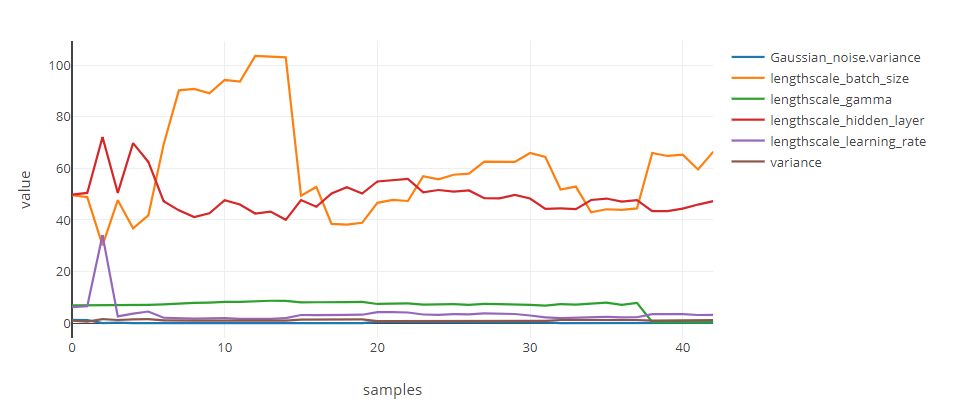
\includegraphics[width=1.0\textwidth]{images/informative-priors.png}
		\caption{Kernel parameters over time in the case of informative priors, where the prior is set based on the hyperparameter range. Parameters almost never rapidly change their value after the initial few samples.}
		\label{figure:informative-priors}
	\end{center}
\end{figure}

\begin{figure}
	\begin{center}
		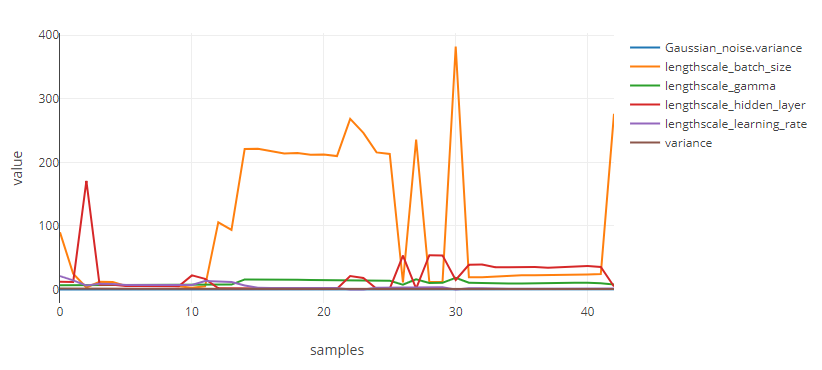
\includegraphics[width=1.0\textwidth]{images/reinforce-jumpy-kernel-params.png}
		\caption{Kernel parameters over time in the case of non-informative priors, where the prior does not depend on the hyperparameter range. Some hyperparameters do not stabilize over time and their scale changes by orders of magnitude.}
		\label{figure:reinforce-jumpy-kernel-params}
	\end{center}
\end{figure}


The informative prior also achieves slightly lower variance than the non-informative one, which matches our intuition of guiding the GP regression model into a more stable area of the kernel parameter space. We confirm this with a kernel parameter visualization as shown in \autoref{figure:informative-priors}, where we can clearly see the parameters to be more stable, than in the case of non-informative priors as shown in \autoref{figure:reinforce-jumpy-kernel-params}.

As a side note, this experiment provided an interesting technical dilemma. Evaluating noisy objective functions is an interesting problem from the practical perspective. Even though the GP regression model is able to model noise in the objective function directly, it can only do so after it is given enough data points which show the noisy trend. But in the context of Bayesian optimization we need to use the model to make decisions about the next evaluation point, even when the number of data points is low. We could run a larger number of evaluations using random search initially, so that the GP could fit the noise in the data. Because of some of the problems with overfitting shown earlier in \autoref{chapter:bo-indepth}, we chose not to model the noise with the model directly, because that could lead to more potential failure points. Instead, we took a practical approach and simply reduced the noise by performing multiple (specifically $20$) evaluations of the REINFORCE model for each set of hyperparameters, and averaged the result. Since this method is a Monte Carlo approximation of the true objective function, its variance decreases as such (roughly as $\frac{1}{\sqrt{N}}$), the GP will be able to fit the objective function with almost an order of magnitude lower noise parameter.


\section{Tuning on Multiple Treebanks Simultaneously}
\label{section:multiple-treebanks-failed}

\begin{figure}
	\begin{center}
		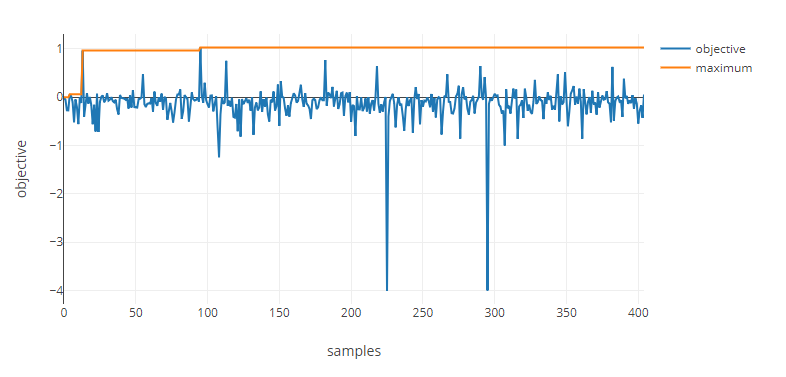
\includegraphics[width=1.0\textwidth]{images/sigmorphon-convergence.png}
		\caption{Convergence plot for a model trained on the SIGMORPHON 2019 shared task. No significant improvement over the baseline was found.}
		\label{figure:sigmorphon-convergence}
	\end{center}
\end{figure}

\begin{figure}
	\begin{center}
		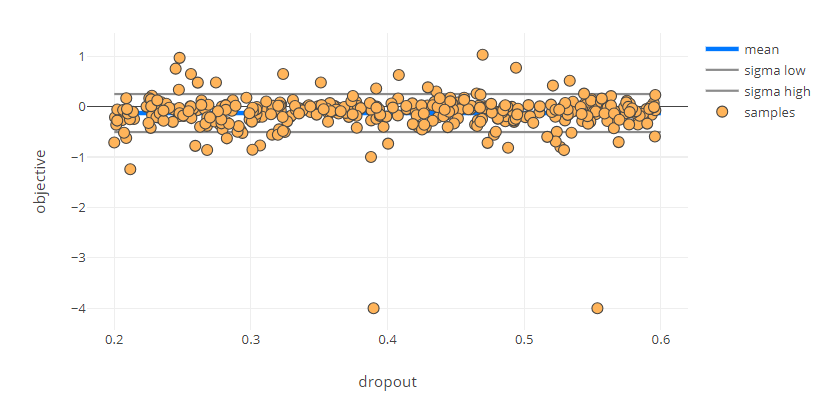
\includegraphics[width=1.0\textwidth]{images/sigmorphon-dropout.png}
		\caption{Marginal regression on the dropout hyperparameter for the SIGMORPHON 2019 shared task when training on all 105 treebanks.}
		\label{figure:sigmorphon-dropout}
	\end{center}
\end{figure}

In this larger experiment we tried to tune hyperparameters for a single model on multiple different datasets at once. Specifically, the model was trained for the SIGMORPHON 2019 shared task 2 \citep{sigmorphon2019task2} on 105 different treebanks, most of which are different languages.\footnote{The shared task training data consists of 107 treebanks, but we did not consider the two largest in the Bayesian optimization for performance reasons.} Our goal was to ideally find one set of hyperparameters that would work well across all of these treebanks. Even though this experiment was not ultimately successful, we still include it in the text as the problem being solved poses interesting technical challenges from the perspective of hyperparameter tuning.

As a fundamental problem of this task, each treebank is of different size, and the difficulty of different languages varies a lot. To give a few specific examples, on Tamil the model achieves around 95\% accuracy in tagging, while on Sanskrit it achieves only 65\%. This makes it nearly impossible to set the objective function to simply be the accuracy of the model, as the same value of hyperparameters could result in the objective varying by 30\%.

We work around this problem by computing a baseline accuracy using an existing, hand tuned, model on the same task, pre-computing its score for each treebank with a fixed set of hyperparameters, and then subtracting its value from the accuracy of our tuned model. The objective function then explicitly becomes the improvement over an existing fixed model.

A second problem we had to solve was how to incorporate the 105 treebanks into the optimization procedure. Because training the model takes multiple GPU hours even for the smaller treebanks, we realistically cannot perform more than a few hundred evaluations total. Instead of training the model on all treebanks for each set of hyperparameters, we only train the model on one treebank for each hyperparameter configuration chosen by Bayesian optimization.

This introduces an interesting choice. In theory, we could treat the treebank as a hyperparameter treated explicitly by Bayesian optimization. As the algorithm balances the exploration-exploitation trade-off, it should be able to pick treebanks as needed to better explore the space. But because of the different sizes and difficulties of each treebank, and the inability of Bayesian optimization to treat categorical hyperparameters well, we decided to not take this approach.

Instead, we omit the treebank from the list of hyperparameters, so that the optimizer has no way of modeling it, and provide it as an explicit parameter outside of the scope of the optimizer. In theory, we could also provide the optimizer with a treebank that was used with each evaluation, not allowing it to optimize the treebank when choosing a next point by overriding its choice, but this approach would most likely yield sub-optimal choices by the optimizer, as the samples would be chosen based on a different criteria than what the optimizer considers. Instead, our way of completely removing the treebank parameter from the optimization process will be seen by the optimizer as noise on the output. If it were to evaluate the same hyperparameters multiple times, the evaluation itself would receive a different treebank, and the improvement over the baseline would be different. In effect this captures our desire to find a unique set of hyperparameters that works well across all treebanks.

Unfortunately, our experimental results did not find a significant improvement over the hyperparameters found by hand-tuning the network (see \autoref{figure:sigmorphon-convergence}). One of the reasons is that the size of the treebank affects which hyperparameter combinations result in value of the objective function. An example of using tuning the same model on a larger treebank is shown in \autoref{section:exp-cestina}.

To give a specific example, when the \emph{batch\_size} hyperparameter is set to a larger value, it works well on a larger treebank, but the opposite is true for a smaller treebank, where a smaller \emph{batch\_size} acts as a regularizer. This means our samples at the same batch size will be spread as far as is the objective on all treebanks. Unfortunately, this spread ends up being so large that all of the hyperparameter end up having no visible trend, as no value is clearly better than the others, as shown in \autoref{figure:sigmorphon-dropout}.\todo{MS: V te figure je urizly "dropout" na spodku}


\section{Tagger on a Single Treebank}
\label{section:exp-cestina}


\begin{figure}
	\begin{center}
		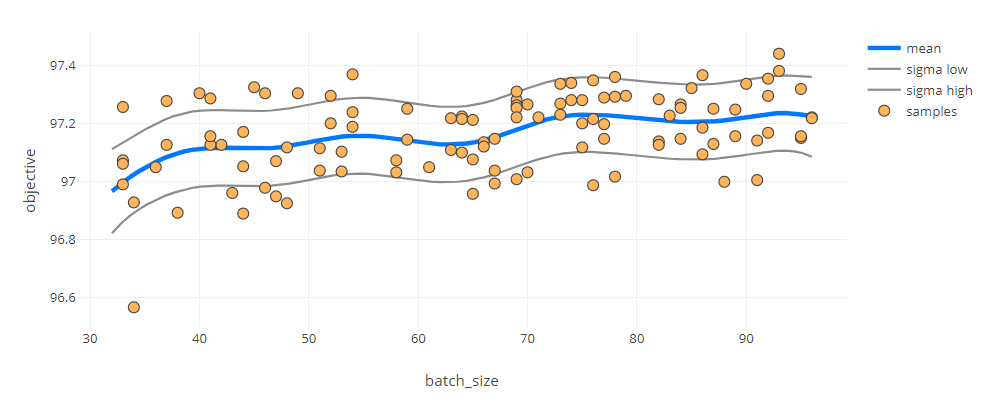
\includegraphics[width=1.0\textwidth]{images/czech-batch-size.png}
		\caption{Marginal regression on the \emph{batch\_size} hyperparameter for the SIGMORPHON 2019 shared task when training on a single Czech treebank.}
		\label{figure:czech-batch-size}
	\end{center}
\end{figure}


\begin{figure}
	\begin{center}
		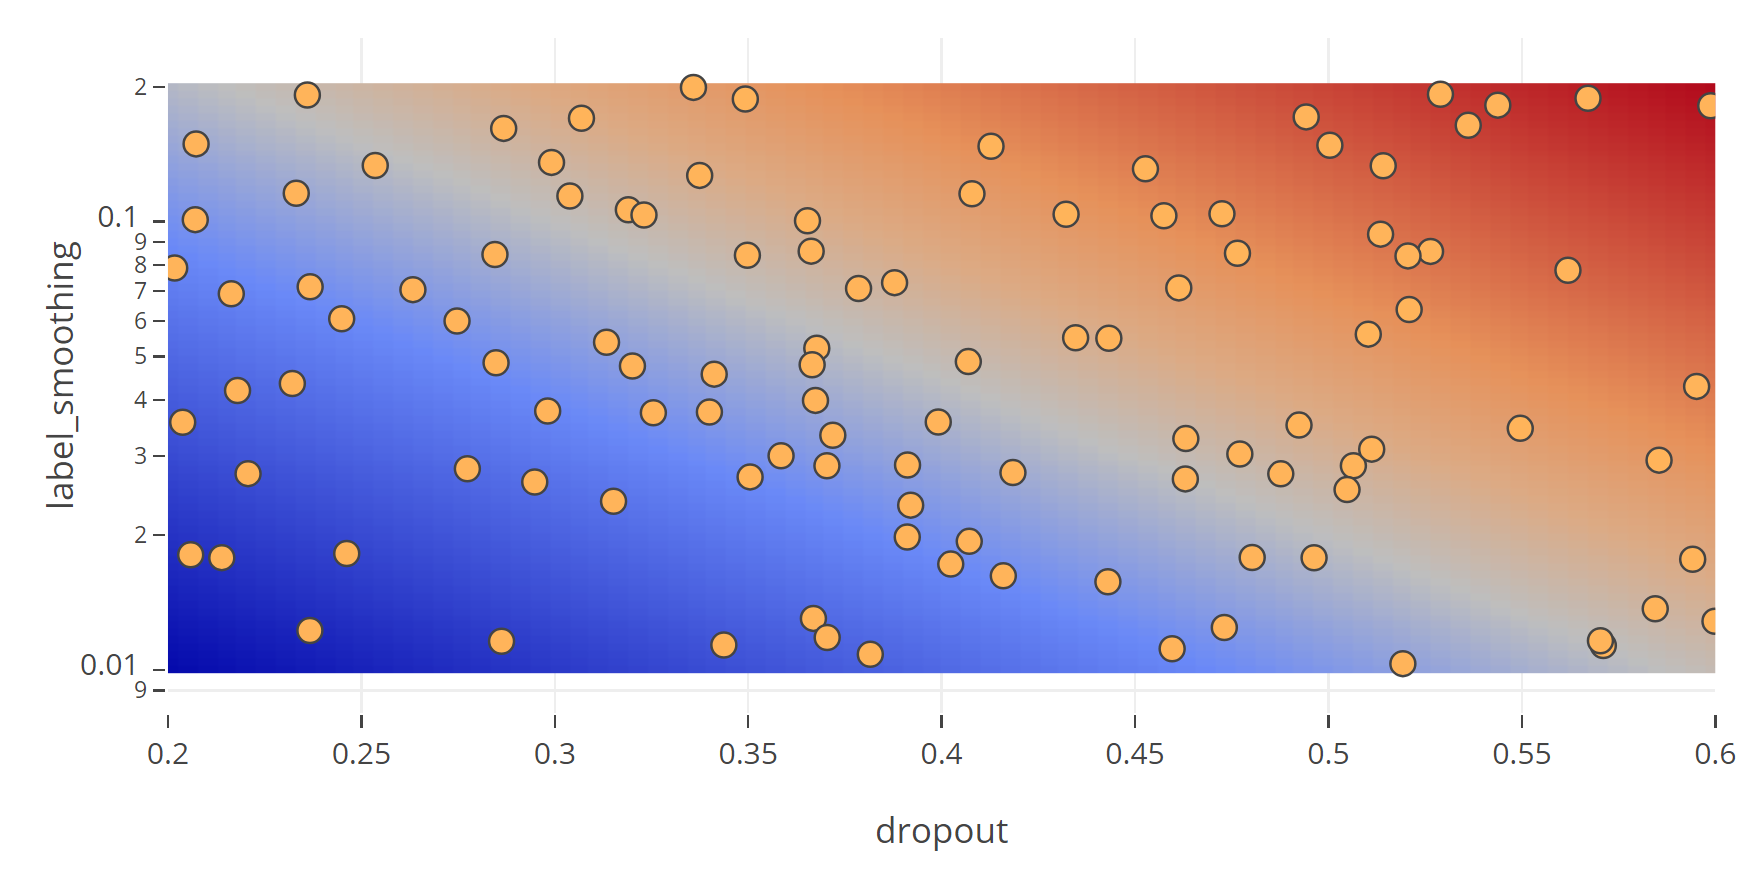
\includegraphics[width=1.0\textwidth]{images/czech-2d-marginal.png}
		\caption{Marginal regression on the \emph{label\_smoothing} and \emph{dropout} hyperparameters for the SIGMORPHON 2019 shared task when training on a single Czech treebank. A correlation between the two parameters is clearly visible, showing that setting only one of them to the correct value is not enough to achieve a high value of the objective function.}
		\label{figure:czech-2d-marginal}
	\end{center}
\end{figure}

Contrary to the experiment shown in \autoref{section:multiple-treebanks-failed} in this experiment we train the same model but only on a single treebank at a time. We tried two different treebanks, Czech and English, which are both quite large. We chose larger treebanks because they provide a more consistent evaluation metric, with the smaller ones being several orders of magnitude smaller, and pose a greater risk of overfitting even on a validation set.

While the previous experiment (see \autoref{section:multiple-treebanks-failed}) did not find any trends in the hyperparameters, the one we present here did find a clear trend in most, as shown for example in \autoref{figure:czech-batch-size}, where larger \emph{batch\_size} is better. In some cases we also found clear relationships between two hyperparameters, such as in the case of \emph{label\_smoothing} and \emph{dropout} shown in \autoref{figure:czech-2d-marginal}.


\section{Other Smaller Experiments}

In this section we briefly show some interesting results from our last two experiments. First, let us show the experiment where we optimized hyperparameters of UDPipe \citep{udpipe:2017} on tokenization of Czech, English and Ancient Greek.

\begin{figure}
	\begin{center}
		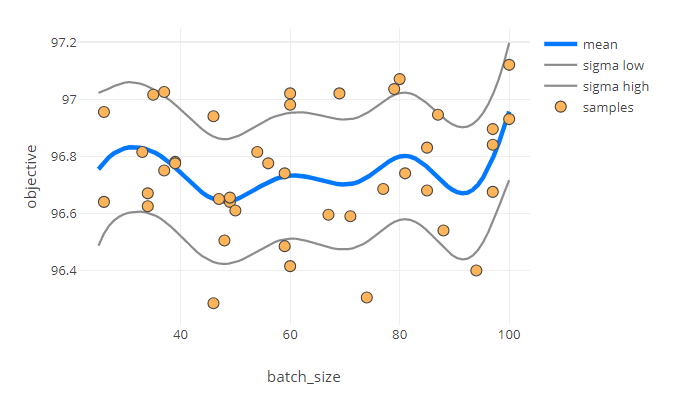
\includegraphics[width=1.0\textwidth]{images/gp-overfitting-batch-size.png}
		\caption{GP regression overfitting on the marginal distribution of \emph{batch\_size}.}
		\label{figure:gp-overfitting-batch-size}
	\end{center}
\end{figure}

Some of the interesting result in this case are the failure cases of the GP regression, particularly how it can overfit on seemingly uninformative dataset, as shown in \autoref{figure:gp-overfitting-batch-size}. These examples nicely show the high capacity of a GP, which, even when we set informative priors, is able to find a surprising way to fit the data with high likelihood. Despite these problems, the Bayesian optimization approach still managed to find hyperparameter values with an objective very close to that find by an exhaustive grid search. Because of the acquisition function, even if the model overfits and picks a bad sample, it will be able to correct itself right afterwards, as the area that was previously receiving high value of acquisition function was explored.

\begin{figure}
	\begin{center}
		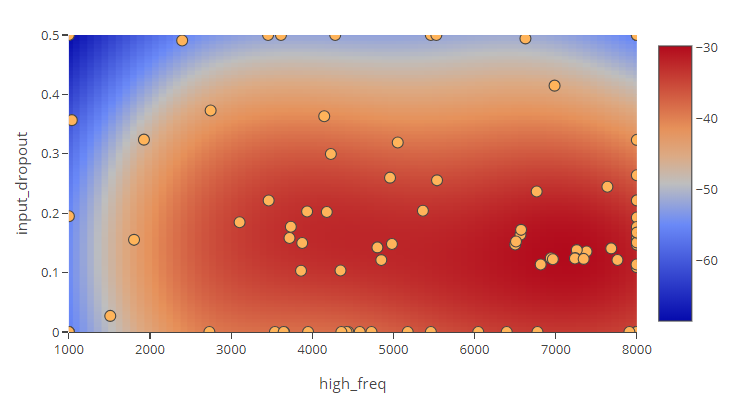
\includegraphics[width=1.0\textwidth]{images/2d-almost-insensitive.png}
		\caption{Marginal 2D regression on the \emph{high\_freq} and \emph{input\_dropout} hyperparameters. The range of the hyperparameters was coincidentally chosen so that only values at the very edge end up with a low value of the objective function, and are indifferent in most of the range.}
		\label{figure:2d-almost-insensitive}
	\end{center}
\end{figure}


As a result, the model still might end up wasting computation time by evaluating incorrect areas by overfitting on the data, but we have not observed it to get stuck in a local optima. Because Bayesian optimization explicitly models exploration into its decision making it quite often ends up doing a decent job of exploring most of the search space, as is visible in all of the figures shown in this chapter.

In the second experiment we trained a speech recognition model on a single dataset. The hyperparameters in this case are however not only the parameters of the model itself, but of a pre-processing step that takes place right before the network is trained. In order to keep the number of hyperparameters lower we fix some of the network's hyperparameters to hand-tuned values, and optimize the ones that have a high chance of being influenced by the preprocessing, such as \emph{batch\_size} and \emph{dropout}.

\autoref{figure:2d-almost-insensitive} shows an example where we coincidentally chose the hyperparameter ranges such that only the values at the very edge have some influence over the objective function. If we were to set them only a little differently the regression could end up showing no relationship between the two hyperparameters. Setting the bounds on hyperparameters is an important but non-trivial effort. If we set the bounds too large, we end up wasting lots of computation time, as the volume of an $n$-dimensional hypercube grows exponentially. On the other hand, if we set the bounds too tight, the optimizer might only find flat regions of the objective function.




\chapter{Conclusion}

- future work

- pribalit vysledky experimentu a jak jednoduse pustit web
